\chapter{Szerver oldali folyamatok implementációi}

A megjelenítési réteg alatt található szerveroldali folyamatok implementációja során a kiszolgáló infrastruktúra kialakítására, a Node.js alkalmazás fejlesztésére, a konténerizált környezet kialakítására, valamint a videófeldolgozásra fókuszálunk ebben a fejezetben.

\section{A virtuális privát felhő komponensei}

TODO: A VPC-beli (Virtual Private Cloud) subnetek, a security groupok, route táblák. A biztonság vizsgálata.

\begin{figure}[ht]
  \centering
  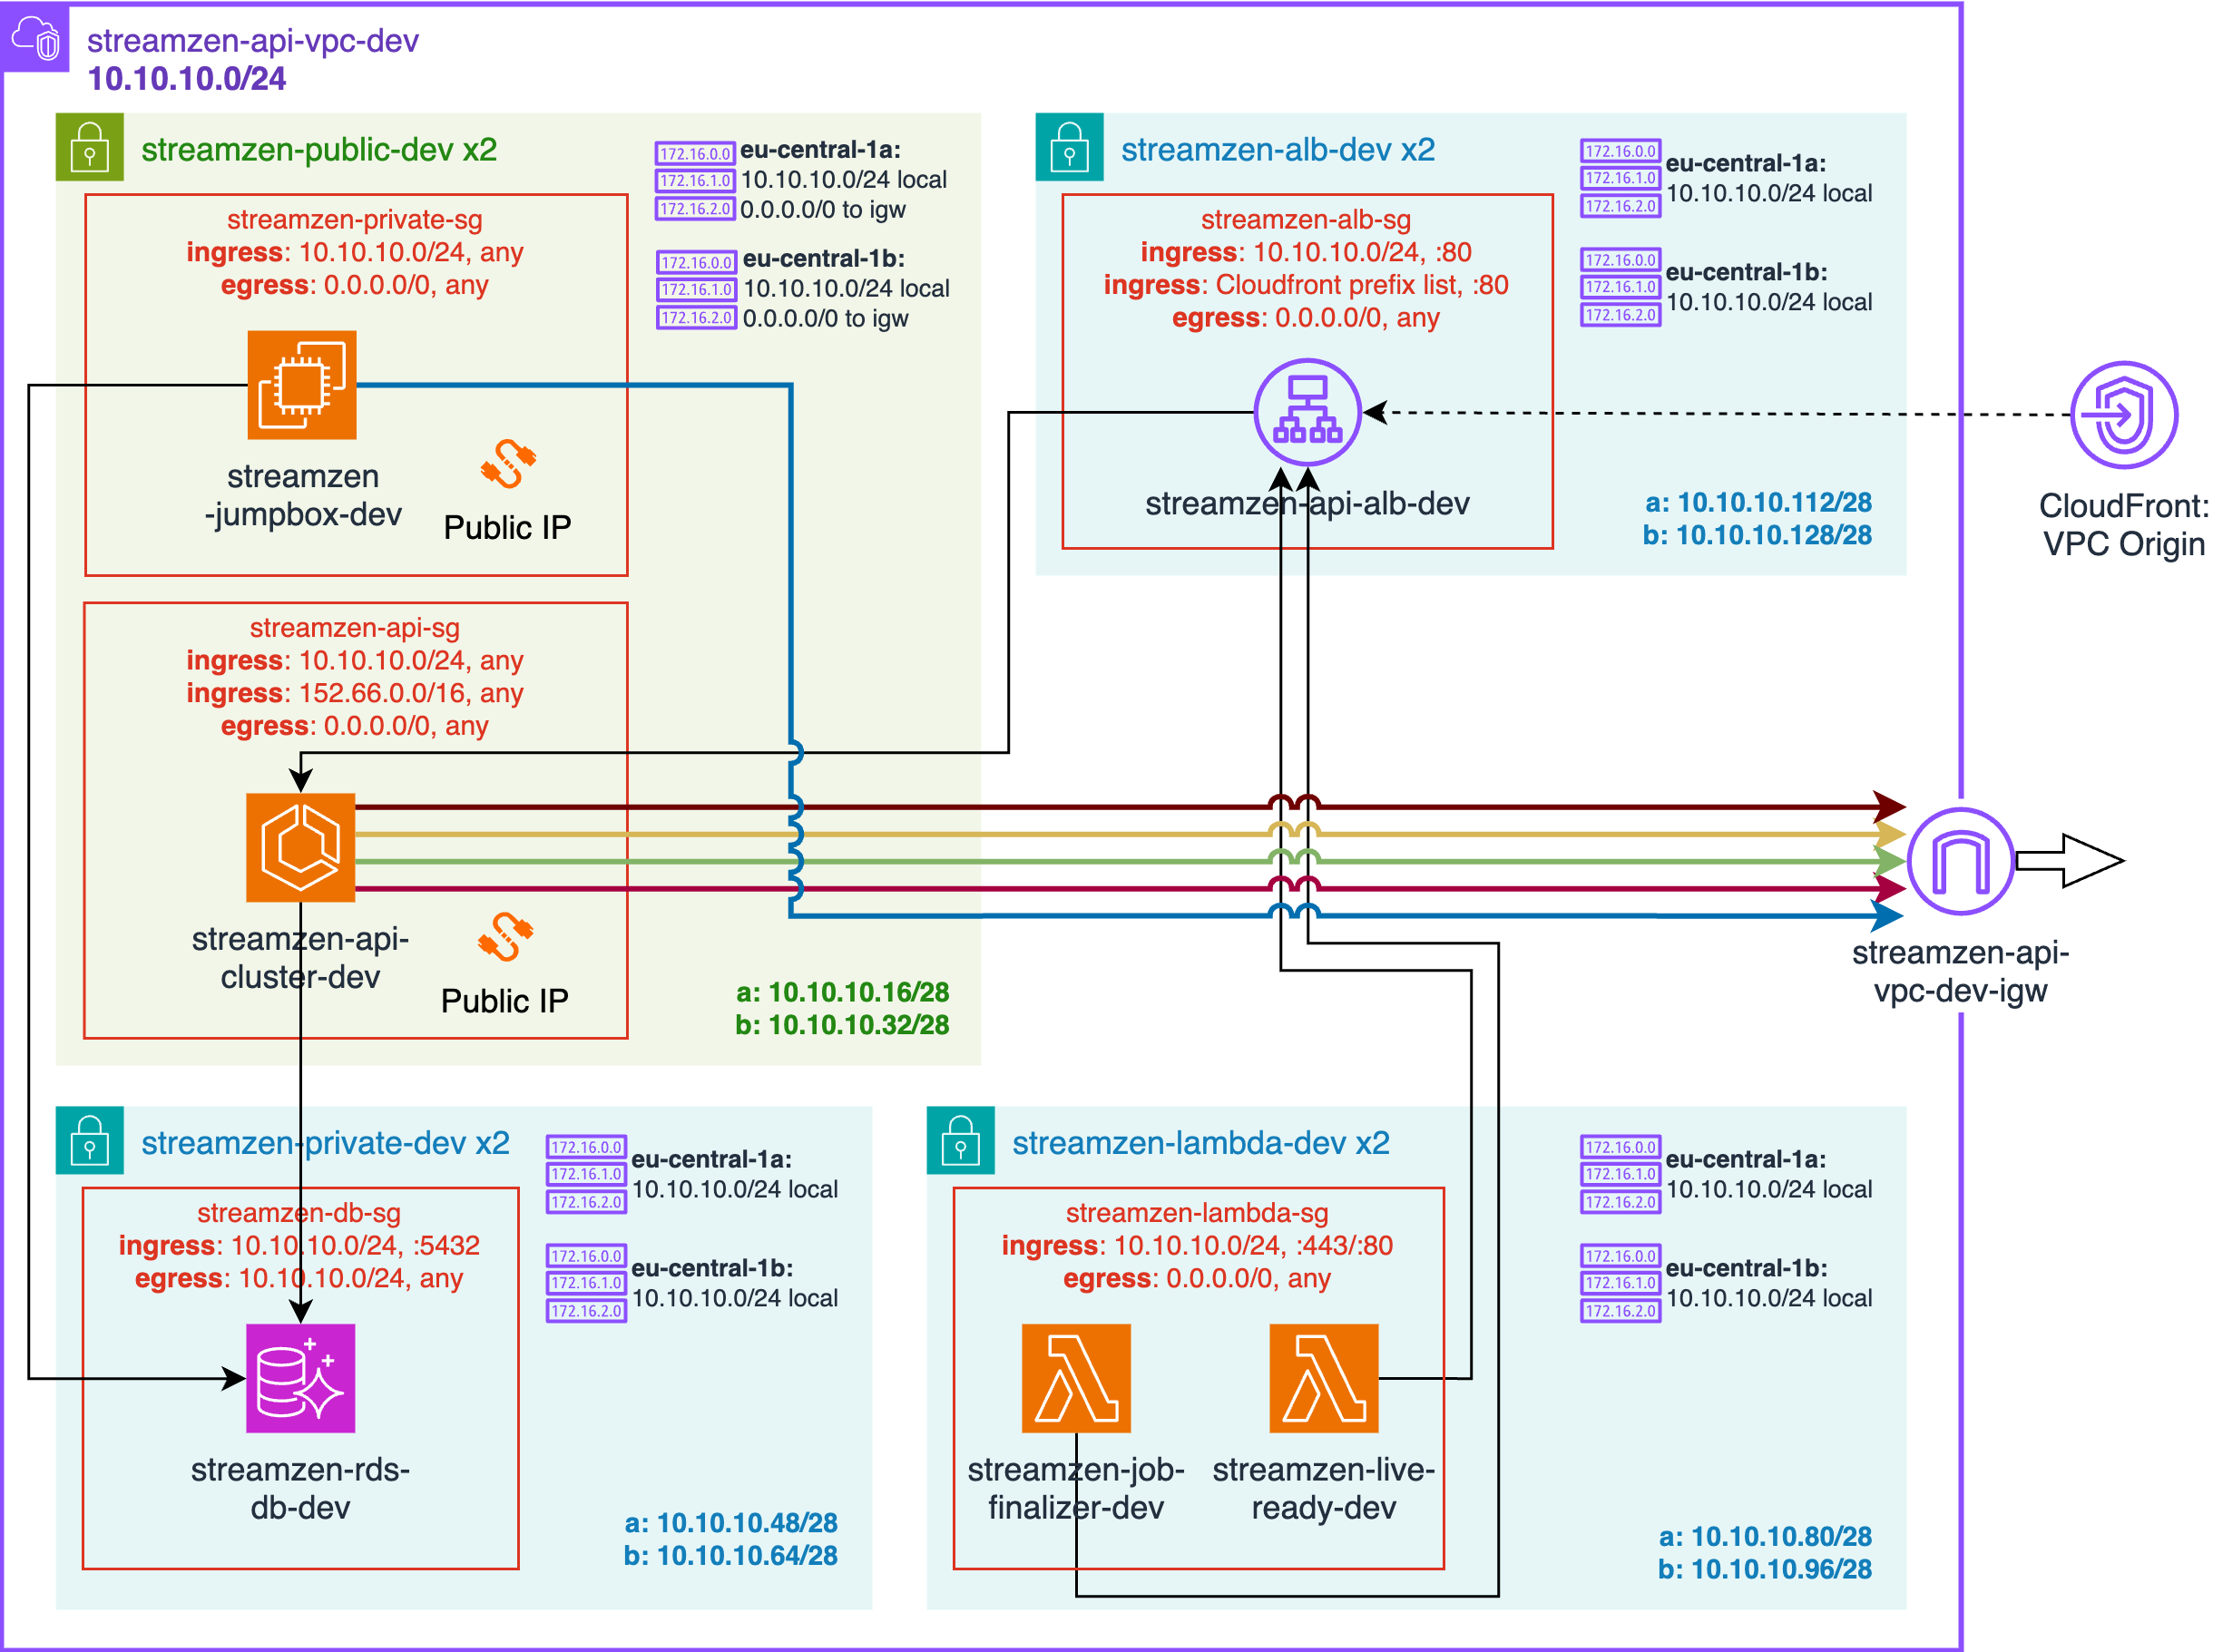
\includegraphics[width=150mm, keepaspectratio]{figures/dipterv_vpc.png}
  \caption{Részletes architektúraábra a VPC-ről.}
  \label{fig:vpc}
\end{figure}

\begin{figure}[ht]
  \centering
  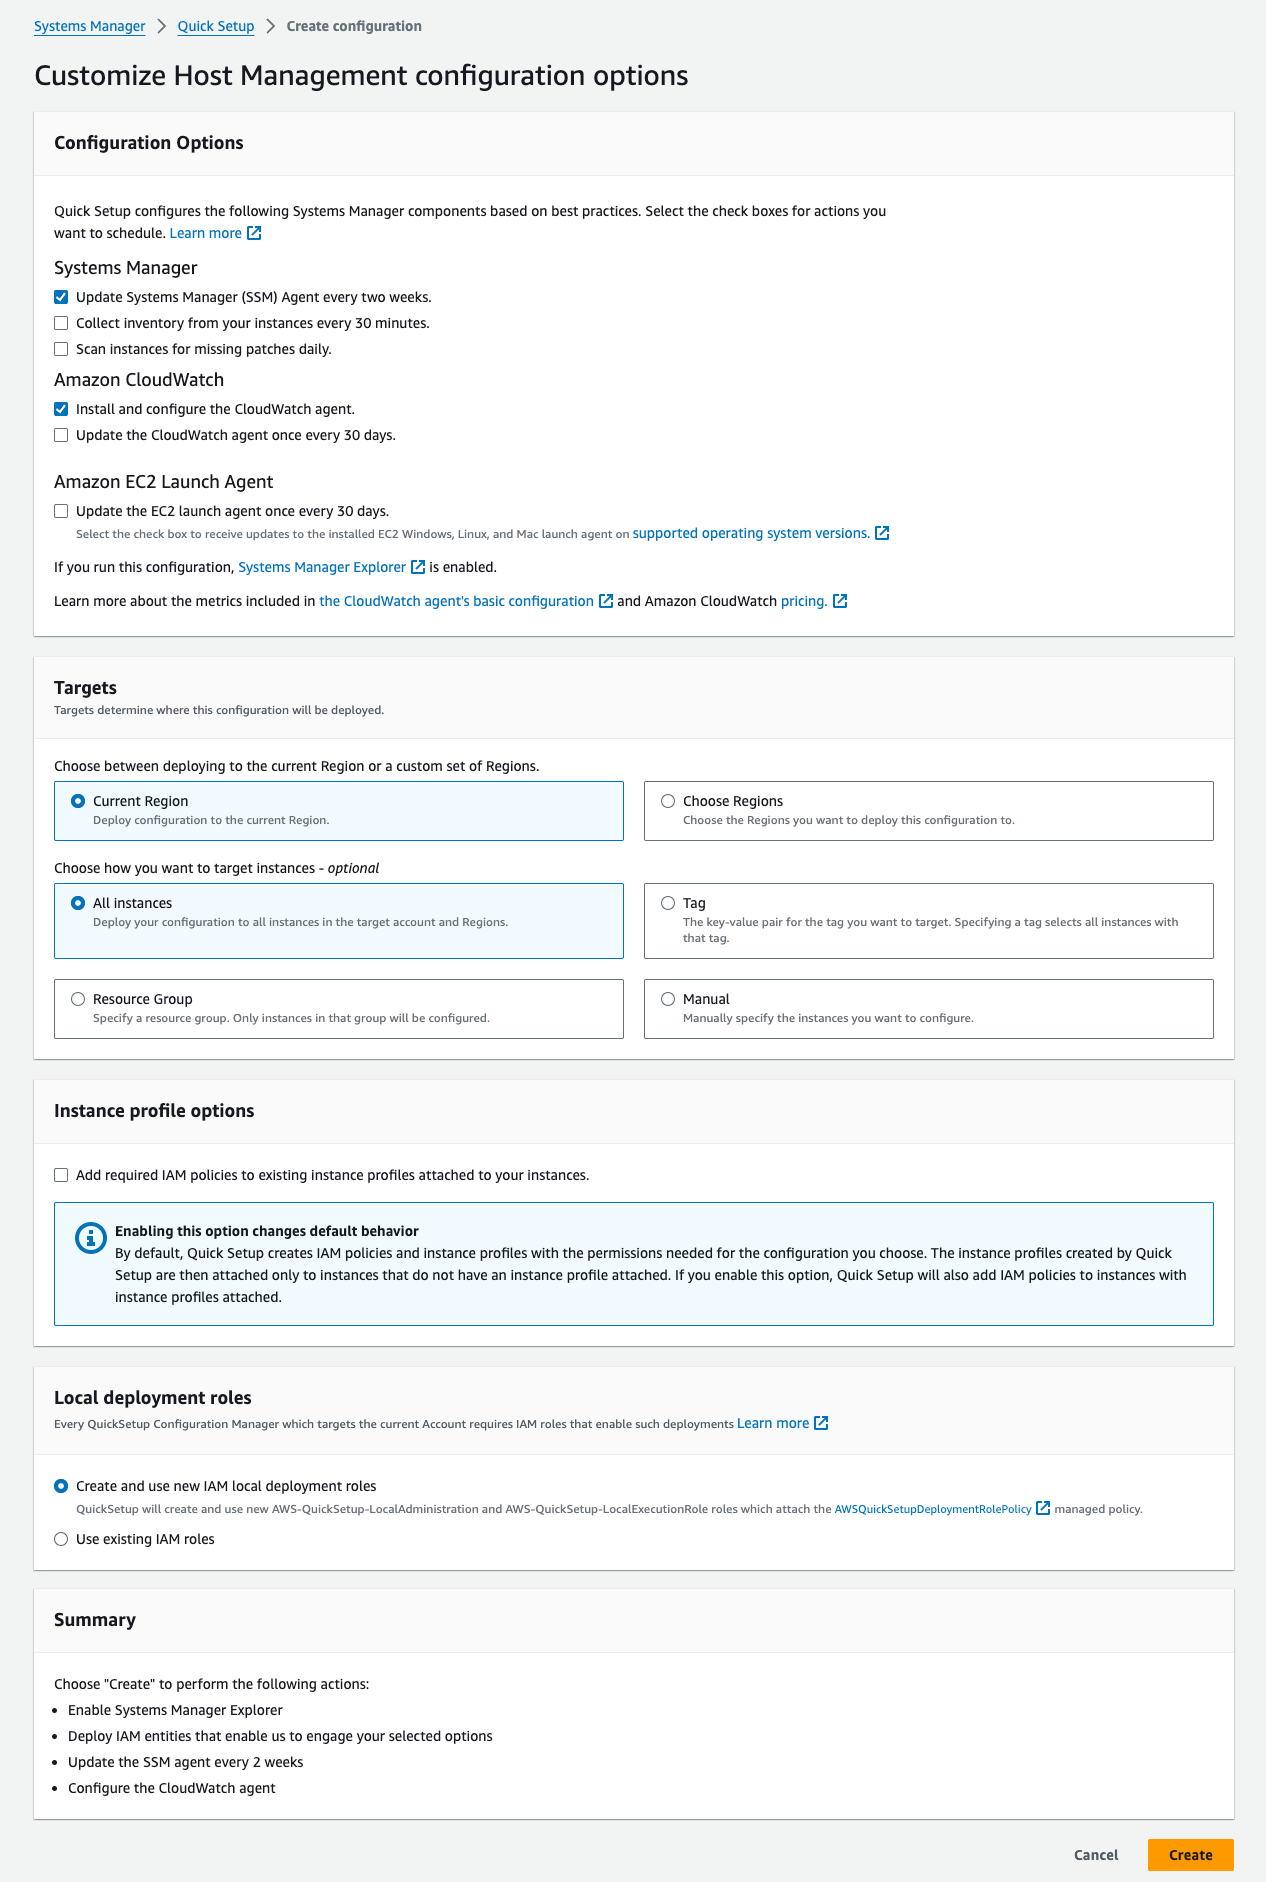
\includegraphics[width=152mm, keepaspectratio]{figures/hostmgmt.png}
  \caption{A Host Management gyorstelepítési oldala.}
  \label{fig:hostmgmt}
\end{figure}

\section{A Node.js alkalmazás fejlesztése}

TODO: Az elkészült alkalmazás felépítése, a különböző rétegek, a routing, a middleware-ek, a kontrollerek, a service-ek, a REST API.

TODO: Itt lehet szó az adatbázisbeli entitásokról is.

TODO: Kódrészletei. Kitérve arra, hogy miképp könnyíti a munkát a Prisma, milyen egyéb szolgáltatások kerültek be, mi a felépítése a reponak, miért választottam ezt a stacket.

TODO: S3 bucketba való mentése a videónak egy érdekes rész.

\section{A konténerizált környezet}

TODO: Leírás, hogy miért választottam a konténerizált környezetet, a konténerizálás előnyeit, hátrányait. Hogy használható ki a legjobban a konténerizáció az Application Load Balancer-rel együtt. Miképp kapcsoltam ezt a kettőt össze (ECS service, ALB).

\subsection{A Node.js szerveralkalmazás ECS-en}

TODO: Az ECS orkesztrációs toolsetjének kialakítása, a konténer rétegződés felépítése ECS-ben, a konténer registry (ECR) bekötése. Környezeti változók, portok, ALB-re való kötése. Miből állt a dockerizálás nekem (Dockerfile, registry, image build, push, networking).

TODO: Milyen IAM role-okat kellett feltenni rá, mikkel kommunikál kifelé, mi indokolta, hogy publikus subnetbe kerüljön. Hogy hív meg más külső rácsatlakozó erőforrásokat (S3 bucket, RDS instance, Lambda függvény, MediaLive channel).

TODO: Jumpbox használata, illetve miért került ki, hol volt egy hibázás a Dockerfile-lal.

\subsection{A szerveralkalmazás CI/CD folyamatai}

TODO: GitHub Actions a smoke tesztre, a deploymentre: Docker build és ECR-be telepítés.

\section{Elemental MediaConvert felhasználása}

TODO: Az Elemental MediaConvert API használata a Lambdából, illetve hogy hogy hívódik meg a Lambda, milyen triggerrel, milyen környezeti változókkal, milyen IAM role-al. Hogy kellett felkonfigurálni a MediaConvert job, hogy kellett magát a Lambdát felkonfigolni, hogy tudja is hívni.
